 % use the "wcp" class option for workshop and conference
 % proceedings
 %\documentclass[gray]{jmlr} % test grayscale version
 \documentclass[tablecaption=bottom]{jmlr}% journal article
 %\documentclass[tablecaption=bottom,wcp]{jmlr} % W&CP article

 % The following packages will be automatically loaded:
 % amsmath, amssymb, natbib, graphicx, url, algorithm2e

 %\usepackage{rotating}% for sideways figures and tables
 %\usepackage{longtable}% for long tables

 % The booktabs package is used by this sample document
 % (it provides \toprule, \midrule and \bottomrule).
 % Remove the next line if you don't require it.
\usepackage{booktabs}
 % The siunitx package is used by this sample document
 % to align numbers in a column by their decimal point.
 % Remove the next line if you don't require it.
\usepackage[load-configurations=version-1]{siunitx} % newer version
 %\usepackage{siunitx}
\usepackage{multirow}

\usepackage{tikz,pgfplots}%,pgfplots,color,amsmath,amssymb}
%\usepackage{caption}
%\usepackage{subcaption}
\usepackage[capitalise]{cleveref}

 % The following command is just for this sample document:
\newcommand{\cs}[1]{\texttt{\char`\\#1}}% remove this in your real article

 % Define an unnumbered theorem just for this sample document for
 % illustrative purposes:
\theorembodyfont{\upshape}
\theoremheaderfont{\scshape}
\theorempostheader{:}
\theoremsep{\newline}
\newtheorem*{note}{Note}

 % change the arguments, as appropriate, in the following:
\jmlrvolume{1}
\jmlryear{2010}
\jmlrsubmitted{submission date}
\jmlrpublished{publication date}
\jmlrworkshop{workshop title} % W&CP title

 % The optional argument of \title is used in the header
\title[Short Title]{Full Title of Article\titlebreak This Title Has
A Line Break}

 % Anything in the title that should appear in the main title but 
 % not in the article's header or the volume's table of
 % contents should be placed inside \titletag{}

 %\title{Title of the Article\titletag{\thanks{Some footnote}}}


 % Use \Name{Author Name} to specify the name.
 % If the surname contains spaces, enclose the surname
 % in braces, e.g. \Name{John {Smith Jones}} similarly
 % if the name has a "von" part, e.g \Name{Jane {de Winter}}.
 % If the first letter in the forenames is a diacritic
 % enclose the diacritic in braces, e.g. \Name{{\'E}louise Smith}

 % \thanks must come after \Name{...} not inside the argument for
 % example \Name{John Smith}\nametag{\thanks{A note}} NOT \Name{John
 % Smith\thanks{A note}}

 % Anything in the name that should appear in the title but not in the 
 % article's header or footer or in the volume's
 % table of contents should be placed inside \nametag{}

 % Two authors with the same address
  \author{\Name{Author Name1\nametag{\thanks{A note}}} \Email{abc@sample.com}\and
   \Name{Author Name2} \Email{xyz@sample.com}\\
   \addr Address}

 % Three or more authors with the same address:
 % \author{\Name{Author Name1} \Email{an1@sample.com}\\
 %  \Name{Author Name2} \Email{an2@sample.com}\\
 %  \Name{Author Name3} \Email{an3@sample.com}\\
 %  \Name{Author Name4} \Email{an4@sample.com}\\
 %  \Name{Author Name5} \Email{an5@sample.com}\\
 %  \Name{Author Name6} \Email{an6@sample.com}\\
 %  \Name{Author Name7} \Email{an7@sample.com}\\
 %  \Name{Author Name8} \Email{an8@sample.com}\\
 %  \Name{Author Name9} \Email{an9@sample.com}\\
 %  \Name{Author Name10} \Email{an10@sample.com}\\
 %  \Name{Author Name11} \Email{an11@sample.com}\\
 %  \Name{Author Name12} \Email{an12@sample.com}\\
 %  \Name{Author Name13} \Email{an13@sample.com}\\
 %  \Name{Author Name14} \Email{an14@sample.com}\\
 %  \addr Address}


 % Authors with different addresses:
 % \author{\Name{Author Name1} \Email{abc@sample.com}\\
 % \addr Address 1
 % \AND
 % \Name{Author Name2} \Email{xyz@sample.com}\\
 % \addr Address 2
 %}

\editor{Editor's name}
 %\editors{Editor One and Editor Two}% for multiple editors

\begin{document}

\maketitle

\begin{abstract}
This is the abstract for this article.
\end{abstract}
\begin{keywords}
List of keywords
\end{keywords}

%\section{Introduction}
\label{sec:intro}

This is a sample article that uses the \textsf{jmlr} class with
the \texttt{wcp} class option.  Please follow the guidelines in
this sample document as it can help to reduce complications when
combining the articles into a book. Please avoid using obsolete
commands, such as \verb|\rm|, and obsolete packages, such as
\textsf{epsfig}.\footnote{See
\url{http://www.ctan.org/pkg/l2tabu}} Some packages that are known
to cause problems for the production editing process are checked for
by the \textsf{jmlr} class and will generate an error.

Please also ensure that your document will compile with PDF\LaTeX.
If you have an error message that's puzzling you, first check for it
at the UK TUG FAQ
\url{https://texfaq.org/FAQ-man-latex}.  If
that doesn't help, create a minimal working example (see
\url{https://www.dickimaw-books.com/latex/minexample/}) and post
to somewhere like \TeX\ on StackExchange
(\url{https://tex.stackexchange.com/}) or the \LaTeX\ Community Forum
(\url{https://latex.org/forum/}).

\begin{note}
This is an numbered theorem-like environment that was defined in
this document's preamble.
\end{note}

\subsection{Sub-sections}

Sub-sections are produced using \verb|\subsection|.

\subsubsection{Sub-sub-sections}

Sub-sub-sections are produced using \verb|\subsubsection|.

\paragraph{Sub-sub-sub-sections}

Sub-sub-sub-sections are produced using \verb|\paragraph|.
These are unnumbered with a running head.

\subparagraph{Sub-sub-sub-sub-sections}

Sub-sub-sub-sub-sections are produced using \verb|\subparagraph|.
These are unnumbered with a running head.

\section{Cross-Referencing}

Always use \verb|\label| and \verb|\ref| (or one of the commands
described below) when cross-referencing.  For example, the next
section is Section~\ref{sec:math} but you can also refer to it using
\sectionref{sec:math}. The \textsf{jmlr} class
provides some convenient cross-referencing commands:
\verb|\sectionref|, \verb|\equationref|, \verb|\tableref|,
\verb|\figureref|, \verb|\algorithmref|, \verb|\theoremref|,
\verb|\lemmaref|, \verb|\remarkref|, \verb|\corollaryref|,
\verb|\definitionref|, \verb|\conjectureref|, \verb|\axiomref|,
\verb|\exampleref| and \verb|\appendixref|. The argument of these
commands may either be a single label or a comma-separated list
of labels. Examples:

Referencing sections: \sectionref{sec:math} or
\sectionref{sec:intro,sec:math} or
\sectionref{sec:intro,sec:math,sec:tables,sec:figures}.

Referencing equations: \equationref{eq:trigrule} or
\equationref{eq:trigrule,eq:df} or
\equationref{eq:trigrule,eq:f,eq:df,eq:y}.

Referencing tables: \tableref{tab:operatornames} or
\tableref{tab:operatornames,tab:example} or
\tableref{tab:operatornames,tab:example,tab:example-booktabs}.

Referencing figures: \figureref{fig:nodes} or
\figureref{fig:nodes,fig:teximage} or
\figureref{fig:nodes,fig:teximage,fig:subfigex} or
\figureref{fig:circle,fig:square}.

Referencing algorithms: \algorithmref{alg:gauss} or
\algorithmref{alg:gauss,alg:moore} or
\algorithmref{alg:gauss,alg:moore,alg:net}.

Referencing theorem-like environments: \theoremref{thm:eigenpow},
\lemmaref{lem:sample}, \remarkref{rem:sample}, 
\corollaryref{cor:sample}, \definitionref{def:sample},
\conjectureref{con:sample}, \axiomref{ax:sample} and
\exampleref{ex:sample}.

Referencing appendices: \appendixref{apd:first} or
\appendixref{apd:first,apd:second}.

\section{Equations}
\label{sec:math}

The \textsf{jmlr} class loads the \textsf{amsmath} package, so
you can use any of the commands and environments defined there.
(See the \textsf{amsmath} documentation for further
details.\footnote{Either \texttt{texdoc amsmath} or
\url{http://www.ctan.org/pkg/amsmath}})

Unnumbered single-lined equations should be displayed using
\verb|\[| and \verb|\]|. For example:
\[E = m c^2\]
or you can use the \texttt{displaymath} environment:
\begin{displaymath}
E = m c^2
\end{displaymath}
Numbered single-line equations should be displayed using the
\texttt{equation} environment. For example:
\begin{equation}\label{eq:trigrule}
\cos^2\theta + \sin^2\theta \equiv 1
\end{equation}
This can be referenced using \verb|\label| and \verb|\equationref|.
For example, \equationref{eq:trigrule}.

Multi-lined numbered equations should be displayed using the
\texttt{align} environment.\footnote{For reasons why you 
shouldn't use the obsolete \texttt{eqnarray} environment, see
Lars Madsen, \emph{Avoid eqnarray!} TUGboat 33(1):21--25, 2012.} For example:
\begin{align}
f(x) &= x^2 + x\label{eq:f}\\
f'(x) &= 2x + 1\label{eq:df}
\end{align}
Unnumbered multi-lined equations can be displayed using the
\texttt{align*} environment. For example:
\begin{align*}
f(x) &= (x+1)(x-1)\\
&= x^2 - 1
\end{align*}
If you want to mix numbered with unnumbered lines use the
\texttt{align} environment and suppress unwanted line numbers with
\verb|\nonumber|. For example:
\begin{align}
y &= x^2 + 3x - 2x + 1\nonumber\\
&= x^2 + x + 1\label{eq:y}
\end{align}
An equation that is too long to fit on a single line can be
displayed using the \texttt{split} environment. 
Text can be embedded in an equation using \verb|\text| or
\verb|\intertext| (as used in \theoremref{thm:eigenpow}).
See the \textsf{amsmath} documentation for further details.

\subsection{Operator Names}
\label{sec:op}

Predefined operator names are listed in \tableref{tab:operatornames}.
For additional operators, either use \verb|\operatorname|,
for example $\operatorname{var}(X)$ or declare it with
\verb|\DeclareMathOperator|, for example
\begin{verbatim}
\DeclareMathOperator{\var}{var}
\end{verbatim}
and then use this new command. If you want limits that go above and
below the operator (like \verb|\sum|) use the starred versions
(\verb|\operatorname*| or \verb|\DeclareMathOperator*|).

\begin{table*}[htbp]
\floatconts
  {tab:operatornames}%
  {\caption{Predefined Operator Names (taken from 
   \textsf{amsmath} documentation)}}%
  {%
\begin{tabular}{rlrlrlrl}
\cs{arccos} & $\arccos$ &  \cs{deg} & $\deg$ &  \cs{lg} & $\lg$ &  \cs{projlim} & $\projlim$ \\
\cs{arcsin} & $\arcsin$ &  \cs{det} & $\det$ &  \cs{lim} & $\lim$ &  \cs{sec} & $\sec$ \\
\cs{arctan} & $\arctan$ &  \cs{dim} & $\dim$ &  \cs{liminf} & $\liminf$ &  \cs{sin} & $\sin$ \\
\cs{arg} & $\arg$ &  \cs{exp} & $\exp$ &  \cs{limsup} & $\limsup$ &  \cs{sinh} & $\sinh$ \\
\cs{cos} & $\cos$ &  \cs{gcd} & $\gcd$ &  \cs{ln} & $\ln$ &  \cs{sup} & $\sup$ \\
\cs{cosh} & $\cosh$ &  \cs{hom} & $\hom$ &  \cs{log} & $\log$ &  \cs{tan} & $\tan$ \\
\cs{cot} & $\cot$ &  \cs{inf} & $\inf$ &  \cs{max} & $\max$ &  \cs{tanh} & $\tanh$ \\
\cs{coth} & $\coth$ &  \cs{injlim} & $\injlim$ &  \cs{min} & $\min$ \\
\cs{csc} & $\csc$ &  \cs{ker} & $\ker$ &  \cs{Pr} & $\Pr$
\end{tabular}\par
\begin{tabular}{rlrl}
\cs{varlimsup} & $\varlimsup$ 
& \cs{varinjlim} & $\varinjlim$\\
\cs{varliminf} & $\varliminf$ 
& \cs{varprojlim} & $\varprojlim$
\end{tabular}
}
\end{table*}

\section{Vectors and Sets}
\label{sec:vec}

Vectors should be typeset using \cs{vec}. For example $\vec{x}$.
(The original version of \cs{vec} can also be accessed using
\cs{orgvec}, for example $\orgvec{x}$.)
The \textsf{jmlr} class also provides \cs{set} to typeset a
set. For example $\set{S}$.

\section{Floats}
\label{sec:floats}

Floats, such as figures, tables and algorithms, are moving
objects and are supposed to float to the nearest convenient
location. Please don't force them to go in a particular place. In
general it's best to use the \texttt{htbp} specifier and don't
put the figure or table in the middle of a paragraph (that is
make sure there's a paragraph break above and below the float).
Floats are supposed to have a little extra space above and below
them to make them stand out from the rest of the text. This extra
spacing is put in automatically and shouldn't need modifying.

If your article will later be reprinted in the Challenges for
Machine Learning, please be aware that the CiML books use a
different paper size, so if you want to resize any images use a
scale relative to the line width (\verb|\linewidth|), text width
(\verb|\textwidth|) or text height (\verb|\textheight|).

To ensure consistency, please \emph{don't} try changing the format of the caption by doing
something like:
\begin{verbatim}
\caption{\textit{A Sample Caption.}}
\end{verbatim}
or
\begin{verbatim}
\caption{\em A Sample Caption.}
\end{verbatim}
You can, of course, change the font for individual words or 
phrases, for example:
\begin{verbatim}
\caption{A Sample Caption With Some \emph{Emphasized Words}.}
\end{verbatim}

\subsection{Tables}
\label{sec:tables}

Tables should go in the \texttt{table} environment. Within this
environment use \verb|\floatconts| (defined by \textsf{jmlr})
to set the caption correctly and center the table contents.
The location of the caption depends on the \verb|tablecaption|
setting in the document class options.

\begin{table}[htbp]
 % The first argument is the label.
 % The caption goes in the second argument, and the table contents
 % go in the third argument.
\floatconts
  {tab:example}%
  {\caption{An Example Table}}%
  {\begin{tabular}{ll}
  \bfseries Dataset & \bfseries Result\\
  Data1 & 0.12345\\
  Data2 & 0.67890\\
  Data3 & 0.54321\\
  Data4 & 0.09876
  \end{tabular}}
\end{table}

If you want horizontal rules you can use the \textsf{booktabs}
package which provides the commands \verb|\toprule|, 
\verb|\midrule| and \verb|\bottomrule|. For example, see
\tableref{tab:example-booktabs}.

\begin{table}[hbtp]
\floatconts
  {tab:example-booktabs}
  {\caption{A Table With Horizontal Lines}}
  {\begin{tabular}{ll}
  \toprule
  \bfseries Dataset & \bfseries Result\\
  \midrule
  Data1 & 0.12345\\
  Data2 & 0.67890\\
  Data3 & 0.54321\\
  Data4 & 0.09876\\
  \bottomrule
  \end{tabular}}
\end{table}

If you really want vertical lines as well, you can't use the
\textsf{booktabs} commands as there'll be some unwanted gaps.
Instead you can use \LaTeX's \verb|\hline|, but the rows may
appear a bit cramped.  You can add extra space above or below a
row using \verb|\abovestrut| and \verb|\belowstrut|. For example,
see \tableref{tab:example-hline}. However, you might want to read
the \textsf{booktabs} documentation regarding the use of vertical
lines.

\begin{table}[htbp]
\floatconts
  {tab:example-hline}
  {\caption{A Table With Horizontal and Vertical Lines}}%
  {%
    \begin{tabular}{|l|l|}
    \hline
    \abovestrut{2.2ex}\bfseries Dataset & \bfseries Result\\\hline
    \abovestrut{2.2ex}Data1 & 0.12345\\
    Data2 & 0.67890\\
    Data3 & 0.54321\\
    \belowstrut{0.2ex}Data4 & 0.09876\\\hline
    \end{tabular}
  }
\end{table}

If you want to align numbers on their decimal point, you can
use the \textsf{siunitx} package. For example, see
\tableref{tab:example-siunitx}. For further details see the
\textsf{siunitx} documentation\footnote{Either \texttt{texdoc
siunitx} or \url{http://www.ctan.org/pkg/siunitx}}.

\begin{table}[htbp]
\floatconts
  {tab:example-siunitx}
  {\caption{A Table With Numbers Aligned on the Decimal Point}}
  {\begin{tabular}{lS[tabformat=3.5]}
  \bfseries Dataset & {\bfseries Result}\\
  Data1 & 0.12345\\
  Data2 & 10.6789\\
  Data3 & 50.543\\
  Data4 & 200.09876
  \end{tabular}}
\end{table}

If the table is too wide, you can adjust the inter-column
spacing by changing the value of \verb|\tabcolsep|. For
example:
\begin{verbatim}
\setlength{\tabcolsep}{3pt}
\end{verbatim}
If the table is very wide but not very long, you can use the
\texttt{sidewaystable} environment defined in the
\textsf{rotating} package (so use \verb|\usepackage{rotating}|).
If the table is too long to fit on a page, you can use the
\texttt{longtable} environment defined in the \textsf{longtable}
package (so use \verb|\usepackage{longtable}|).

\subsection{Figures}
\label{sec:figures}

Figures should go in the \texttt{figure} environment. Within this
environment, use \verb|\floatconts| to correctly position the
caption and center the image. Use \verb|\includegraphics|
for external graphics files but omit the file extension. Do not
use \verb|\epsfig| or \verb|\psfig|. If you want to scale the
image, it's better to use a fraction of the line width rather
than an explicit length. For example, see \figureref{fig:nodes}.

\begin{figure}[htbp]
 % Caption and label go in the first argument and the figure contents
 % go in the second argument
\floatconts
  {fig:nodes}
  {\caption{Example Image}}
  {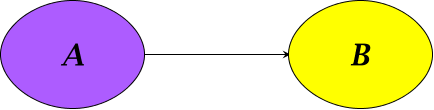
\includegraphics[width=0.5\linewidth]{images/nodes}}
\end{figure}

If your image is made up of \LaTeX\ code (for example, commands
provided by the \textsf{pgf} package) you can include it using
\cs{includeteximage} (defined by the \textsf{jmlr} class). This
can be scaled and rotated in the same way as \cs{includegraphics}.
For example, see \figureref{fig:teximage}.

\begin{figure}[htbp]
\floatconts
  {fig:teximage}
  {\caption{Image Created Using \LaTeX\ Code}}
  {\includeteximage[angle=45]{images/teximage}}
\end{figure}

If the figure is too wide to fit on the page, you can use the
\texttt{sidewaysfigure} environment defined in the
\textsf{rotating} package.

Don't use \verb|\graphicspath|.\footnote{This is specific to the
\textsf{jmlr} class, not a general recommendation. The main file
that generates the proceedings or the CiML book is typically in a
different directory to the imported articles, so it modifies the
graphics path when it imports an article.} If the images 
are contained in a subdirectory, specify this when you include the image, for
example \verb|\includegraphics{figures/mypic}|.

\subsubsection{Sub-Figures}
\label{sec:subfigures}

Sub-figures can be created using \verb|\subfigure|, which is
defined by the \textsf{jmlr} class. The optional argument allows
you to provide a subcaption. The label should be placed in the
mandatory argument of \verb|\subfigure|. You can reference the
entire figure, for example \figureref{fig:subfigex}, or you can
reference part of the figure using \verb|\figureref|, for example
\figureref{fig:circle}. Alternatively you can reference the
subfigure using \verb|\subfigref|, for example
\subfigref{fig:circle,fig:square} in \figureref{fig:subfigex}.

\begin{figure}[htbp]
\floatconts
  {fig:subfigex}
  {\caption{An Example With Sub-Figures.}}
  {%
    \subfigure[A Circle]{\label{fig:circle}%
      
\includegraphics[width=0.2\linewidth]{images/circle}}%
    \qquad
    \subfigure[A Square]{\label{fig:square}%
      
\includegraphics[width=0.2\linewidth]{images/square}}
  }
\end{figure}

By default, the sub-figures are aligned on the baseline.
This can be changed using the second optional argument
of \verb|\subfigure|. This may be \texttt{t} (top), \texttt{c}
(centered) or \texttt{b} (bottom). For example, the subfigures
\subfigref{fig:circle2,fig:square2} in \figureref{fig:subfigex2}
both have \verb|[c]| as the second optional argument.

\begin{figure}[htbp]
\floatconts
  {fig:subfigex2}
  {\caption{Another Example With Sub-Figures.}}
  {%
    \subfigure[A Small Circle][c]{\label{fig:circle2}%
      
\includegraphics[width=0.1\linewidth]{images/circle}}%
    \qquad
    \subfigure[A Square][c]{\label{fig:square2}%
      
\includegraphics[width=0.2\linewidth]{images/square}}
  }
\end{figure}

\subsection{Sub-Tables}
\label{sec:subtables}
There is an analogous command \verb|\subtable| for sub-tables.
It has the same syntax as \verb|\subfigure| described above.
You can reference the table using \verb|\tableref|, for example
\tableref{tab:subtabex} or you can reference part of the table,
for example \tableref{tab:ab}. Alternatively you can reference the
subtable using \verb|\subtabref|, for example
\subtabref{tab:ab,tab:cd} in \tableref{tab:subtabex}.

\begin{table}[htbp]
\floatconts
 {tab:subtabex}
 {\caption{An Example With Sub-Tables}}
 {%
   \subtable{%
     \label{tab:ab}%
     \begin{tabular}{cc}
     \bfseries A & \bfseries B\\
     1 & 2
     \end{tabular}
   }\qquad
   \subtable{%
     \label{tab:cd}%
     \begin{tabular}{cc}
     \bfseries C & \bfseries D\\
     3 & 4\\
     5 & 6
     \end{tabular}
   }
 }
\end{table}

By default, the sub-tables are aligned on the top.
This can be changed using the second optional argument
of \verb|\subtable|. This may be \texttt{t} (top), \texttt{c}
(centered) or \texttt{b} (bottom). For example, the sub-tables
\subtabref{tab:ab2,tab:cd2} in \tableref{tab:subtabex2}
both have \verb|[c]| as the second optional argument.

\begin{table}[htbp]
\floatconts
 {tab:subtabex2}
 {\caption{Another Example With Sub-Tables}}
 {%
   \subtable[][c]{%
     \label{tab:ab2}%
     \begin{tabular}{cc}
     \bfseries A & \bfseries B\\
     1 & 2
     \end{tabular}
   }\qquad
   \subtable[][c]{%
     \label{tab:cd2}%
     \begin{tabular}{cc}
     \bfseries C & \bfseries D\\
     3 & 4\\
     5 & 6
     \end{tabular}
   }
 }
\end{table}

\subsection{Algorithms}
\label{sec:algorithms}

Enumerated textual algorithms can be displayed using the
\texttt{algorithm} environment. Within this environment, use
\verb|\caption| to set the caption and you can use an
\texttt{enumerate} or nested \texttt{enumerate} environments.
For example, see \algorithmref{alg:gauss}. Note that algorithms
float like figures and tables.

\begin{algorithm}[htbp]
\floatconts
  {alg:gauss}%
  {\caption{The Gauss-Seidel Algorithm}}%
{%
\begin{enumerate}
  \item For $k=1$ to maximum number of iterations
    \begin{enumerate}
      \item For $i=1$ to $n$
        \begin{enumerate}
        \item $x_i^{(k)} = 
          \frac{b_i - \sum_{j=1}^{i-1}a_{ij}x_j^{(k)}
          - \sum_{j=i+1}^{n}a_{ij}x_j^{(k-1)}}{a_{ii}}$
        \item If $\|\vec{x}^{(k)}-\vec{x}^{(k-1)} < \epsilon\|$,
          where $\epsilon$ is a specified stopping criteria, stop.
      \end{enumerate}
    \end{enumerate}
\end{enumerate}
}%
\end{algorithm}

If you'd rather have the same numbering throughout the algorithm
but still want the convenient indentation of nested 
\texttt{enumerate} environments, you can use the
\texttt{enumerate*} environment provided by the \textsf{jmlr}
class. For example, see \algorithmref{alg:moore}.

\begin{algorithm}
\floatconts
  {alg:moore}%
  {\caption{Moore's Shortest Path}}%
{%
Given a connected graph $G$, where the length of each edge is 1:
\begin{enumerate*}
  \item Set the label of vertex $s$ to 0
  \item Set $i=0$
  \begin{enumerate*}
    \item \label{step:locate}Locate all unlabelled vertices 
          adjacent to a vertex labelled $i$ and label them $i+1$
    \item If vertex $t$ has been labelled,
    \begin{enumerate*}
      \item[] the shortest path can be found by backtracking, and 
      the length is given by the label of $t$.
    \end{enumerate*}
    otherwise
    \begin{enumerate*}
      \item[] increment $i$ and return to step~\ref{step:locate}
    \end{enumerate*}
  \end{enumerate*}
\end{enumerate*}
}%
\end{algorithm}

Pseudo code can be displayed using the \texttt{algorithm2e}
environment. This is defined by the \textsf{algorithm2e} package
(which is automatically loaded) so check the \textsf{algorithm2e}
documentation for further details.\footnote{Either \texttt{texdoc
algorithm2e} or \url{http://www.ctan.org/pkg/algorithm2e}}
For an example, see \algorithmref{alg:net}.

\begin{algorithm2e}
\caption{Computing Net Activation}
\label{alg:net}
 % older versions of algorithm2e have \dontprintsemicolon instead
 % of the following:
 %\DontPrintSemicolon
 % older versions of algorithm2e have \linesnumbered instead of the
 % following:
 %\LinesNumbered
\KwIn{$x_1, \ldots, x_n, w_1, \ldots, w_n$}
\KwOut{$y$, the net activation}
$y\leftarrow 0$\;
\For{$i\leftarrow 1$ \KwTo $n$}{
  $y \leftarrow y + w_i*x_i$\;
}
\end{algorithm2e}

\section{Description Lists}

The \textsf{jmlr} class also provides a description-like 
environment called \texttt{altdescription}. This has an
argument that should be the widest label in the list. Compare:
\begin{description}
\item[add] A method that adds two variables.
\item[differentiate] A method that differentiates a function.
\end{description}
with
\begin{altdescription}{differentiate}
\item[add] A method that adds two variables.
\item[differentiate] A method that differentiates a function.
\end{altdescription}

\section{Theorems, Lemmas etc}
\label{sec:theorems}

The following theorem-like environments are predefined by
the \textsf{jmlr} class: \texttt{theorem}, \texttt{example},
\texttt{lemma}, \texttt{proposition}, \texttt{remark}, 
\texttt{corollary}, \texttt{definition}, \texttt{conjecture}
and \texttt{axiom}. You can use the \texttt{proof} environment
to display the proof if need be, as in \theoremref{thm:eigenpow}.

\begin{theorem}[Eigenvalue Powers]\label{thm:eigenpow}
If $\lambda$ is an eigenvalue of $\vec{B}$ with eigenvector
$\vec{\xi}$, then $\lambda^n$ is an eigenvalue of $\vec{B}^n$
with eigenvector $\vec{\xi}$.
\begin{proof}
Let $\lambda$ be an eigenvalue of $\vec{B}$ with eigenvector
$\xi$, then
\begin{align*}
\vec{B}\vec{\xi} &= \lambda\vec{\xi}
\intertext{premultiply by $\vec{B}$:}
\vec{B}\vec{B}\vec{\xi} &= \vec{B}\lambda\vec{\xi}\\
\Rightarrow \vec{B}^2\vec{\xi} &= \lambda\vec{B}\vec{\xi}\\
&= \lambda\lambda\vec{\xi}\qquad
\text{since }\vec{B}\vec{\xi}=\lambda\vec{\xi}\\
&= \lambda^2\vec{\xi}
\end{align*}
Therefore true for $n=2$. Now assume true for $n=k$:
\begin{align*}
\vec{B}^k\vec{\xi} &= \lambda^k\vec{\xi}
\intertext{premultiply by $\vec{B}$:}
\vec{B}\vec{B}^k\vec{\xi} &= \vec{B}\lambda^k\vec{\xi}\\
\Rightarrow \vec{B}^{k+1}\vec{\xi} &= \lambda^k\vec{B}\vec{\xi}\\
&= \lambda^k\lambda\vec{\xi}\qquad
\text{since }\vec{B}\vec{\xi}=\lambda\vec{\xi}\\
&= \lambda^{k+1}\vec{\xi}
\end{align*}
Therefore true for $n=k+1$. Therefore, by induction, true for all
$n$.
\end{proof}
\end{theorem}

\begin{lemma}[A Sample Lemma]\label{lem:sample}
This is a lemma.
\end{lemma}

\begin{remark}[A Sample Remark]\label{rem:sample}
This is a remark.
\end{remark}

\begin{corollary}[A Sample Corollary]\label{cor:sample}
This is a corollary.
\end{corollary}

\begin{definition}[A Sample Definition]\label{def:sample}
This is a definition.
\end{definition}

\begin{conjecture}[A Sample Conjecture]\label{con:sample}
This is a conjecture.
\end{conjecture}

\begin{axiom}[A Sample Axiom]\label{ax:sample}
This is an axiom.
\end{axiom}

\begin{example}[An Example]\label{ex:sample}
This is an example.
\end{example}

\section{Color vs Grayscale}
\label{sec:color}

It's helpful if authors supply grayscale versions of their
images in the event that the article is to be incorporated into
a black and white printed book. With external PDF, PNG or JPG
graphic files, you just need to supply a grayscale version of the
file. For example, if the file is called \texttt{myimage.png},
then the gray version should be \texttt{myimage-gray.png} or
\texttt{myimage-gray.pdf} or \texttt{myimage-gray.jpg}. You don't
need to modify your code. The \textsf{jmlr} class checks for
the existence of the grayscale version if it is print mode 
(provided you have used \verb|\includegraphics| and haven't
specified the file extension).

You can use \verb|\ifprint| to determine which mode you are in.
For example, in \figureref{fig:nodes}, the 
\ifprint{dark gray}{purple} ellipse represents an input and the
\ifprint{light gray}{yellow} ellipse represents an output.
Another example: {\ifprint{\bfseries}{\color{red}}important text!}

You can use the class option \texttt{gray} to see how the
document will appear in gray scale mode. \textcolor{blue}{Colored
text} will automatically be converted to gray scale in print mode.

The \textsf{jmlr} class loads the \textsf{xcolor}
package, so you can also define your own colors. For example:
\ifprint
  {\definecolor{myred}{gray}{0.5}}%
  {\definecolor{myred}{rgb}{0.5,0,0}}%
\textcolor{myred}{XYZ}.

The \textsf{xcolor} class is loaded with the \texttt{x11names}
option, so you can use any of the x11 predefined colors (listed
in the \textsf{xcolor} documentation\footnote{either 
\texttt{texdoc xcolor} or \url{http://www.ctan.org/pkg/xcolor}}).

\section{Citations and Bibliography}
\label{sec:cite}

The \textsf{jmlr} class automatically loads \textsf{natbib}
and automatically sets the bibliography style, so you don't need to
use \verb|\bibliographystyle|.
This sample file has the citations defined in the accompanying
BibTeX file \texttt{jmlr-sample.bib}. For a parenthetical
citation use \verb|\citep|. For example
\citep{guyon-elisseeff-03}. For a textual citation use
\verb|\citet|. For example \citet{guyon2007causalreport}. 
Both commands may take a comma-separated list, for example
\citet{guyon-elisseeff-03,guyon2007causalreport}.

These commands have optional arguments and have a starred
version. See the \textsf{natbib} documentation for further
details.\footnote{Either \texttt{texdoc natbib} or
\url{http://www.ctan.org/pkg/natbib}}

The bibliography is displayed using \verb|\bibliography|.

\section{Experimental results}
\label{sec:experiments}

\subsection{Balance dataset}

“Hi Amy! Your mum sent me a text. You forgot your inhaler. Why don’t you turn your phone on?” Amy didn’t like technology. She never sent text messages and she hated Facebook too.

“Did Kamal ask you to the disco?” Tara was Amy’s best friend, and she wanted to know everything that was happening in Amy’s life. “I don’t think he likes me,” said Amy. “And I never see him alone. He’s always with Grant.” Amy and Tara didn’t like Grant.

“Do you know about their art project?” asked Amy. “It’s about graffiti, I think,” said Tara. “They’re working on it at the old house behind the factory.” “But that building is dangerous,” said Amy. “Aah, are you worried he’s going to get hurt?" Tara teased. “Shut up, Tara! Hey look, here they come!”

Kamal and Grant arrived. “Hi Kamal!” said Tara. “Are you going to the Halloween disco tomorrow?” “Yes. Hi Amy,” Kamal said, smiling. “Do you want to come and see our paintings after school?” “I’m coming too!” Tara insisted.

After school, Kamal took the girls to the old house. It was very old and very dirty too. There was rubbish everywhere. The windows were broken and the walls were damp. It was scary. Amy didn’t like it. There were paintings of zombies and skeletons on the walls. “We’re going to take photos for the school art competition,” said Kamal. Amy didn’t like it but she didn’t say anything. “Where’s Grant?” asked Tara. “Er, he’s buying more paint.” Kamal looked away quickly. Tara thought he looked suspicious. “It’s getting dark, can we go now?” said Amy. She didn’t like zombies.

Then, they heard a loud noise coming from a cupboard in the corner of the room. “What’s that?” Amy was frightened. “I didn’t hear anything,” said Kamal. Something was making strange noises. There was something inside the cupboard. “Oh no! What is it?” Amy was very frightened now. “What do you mean? There’s nothing there!” Kamal was trying not to smile. Suddenly the door opened with a bang and a zombie appeared, shouting and moving its arms. Amy screamed and covered her eyes. “Oh very funny, Grant!” said Tara looking bored. Kamal and Grant started laughing. “Ha ha, you were frightened!” said Grant. "Do you like my zombie costume?” Amy took Tara’s arm. “I can’t breathe,” she said. Kamal looked worried now. “Is she OK? It was only a joke.” “No she’s not OK, you idiot. She’s having an asthma attack and she forgot her inhaler.” Tara took out her phone. “I’m calling her dad.”

Next evening was Halloween. The girls were at the school disco. “Are you better now?” asked Tara. “I’m fine,” said Amy. “I think it was the smell of paint that started the attack.” Tara looked around. “So, where are the zombies?” “I don’t know, I don’t want to see Kamal again,” said Amy. “Come on, let’s dance!”

%\begin{figure}[htbp]
%\floatconts
%  {fig:teximage}
%  {\caption{Image Created Using \LaTeX\ Code}}
%  {\includeteximage{plots/balance-dist-class}}
%\end{figure}



\begin{figure}[htbp]
\floatconts
  {fig:balance}
  {\caption{Results for \textit{balance} dataset.}}
  {%
    \subfigure[Distribution between classes]{
    \label{fig:balance:dist-class}%
    \includeteximage{plots/balance-dist-class}
    }%
    \qquad
    \subfigure[Baseline error]{\label{fig:square}%
      \includeteximage{plots/balance-baseline-error}
      }
    \qquad
    \subfigure[$oneC$: SVM and DT]{\label{fig:square}%
      \includeteximage{plots/balance-oneC-0}
      %\includeteximage{plots/balance-dist-class}
      }
    \qquad
    \subfigure[A Square]{\label{fig:square}%
      \includeteximage{plots/balance-avgC-0}
      }
    \qquad
    \subfigure[$oneC$: SVM and DT]{\label{fig:square}%
      \includeteximage{plots/balance-oneC-2}
      }
    \qquad
    \subfigure[A Square]{\label{fig:square}%
      \includeteximage{plots/balance-avgC-2}
      }
    \qquad
    \subfigure[$oneC$: SVM and DT]{\label{fig:square}%
      \includeteximage{plots/balance-oneC-4}
      }
    \qquad
    \subfigure[A Square]{\label{fig:square}%
      \includeteximage{plots/balance-avgC-4}
      }
    \qquad
    \subfigure[$oneC$: SVM and DT]{\label{fig:square}%
      \includeteximage{plots/balance-oneC-6}
      }
    \qquad
    \subfigure[A Square]{\label{fig:square}%
      \includeteximage{plots/balance-avgC-6}
      }
  }
\end{figure}

“Hi Amy! Your mum sent me a text. You forgot your inhaler. Why don’t you turn your phone on?” Amy didn’t like technology. She never sent text messages and she hated Facebook too.

“Did Kamal ask you to the disco?” Tara was Amy’s best friend, and she wanted to know everything that was happening in Amy’s life. “I don’t think he likes me,” said Amy. “And I never see him alone. He’s always with Grant.” Amy and Tara didn’t like Grant.

“Do you know about their art project?” asked Amy. “It’s about graffiti, I think,” said Tara. “They’re working on it at the old house behind the factory.” “But that building is dangerous,” said Amy. “Aah, are you worried he’s going to get hurt?" Tara teased. “Shut up, Tara! Hey look, here they come!”

Kamal and Grant arrived. “Hi Kamal!” said Tara. “Are you going to the Halloween disco tomorrow?” “Yes. Hi Amy,” Kamal said, smiling. “Do you want to come and see our paintings after school?” “I’m coming too!” Tara insisted.

After school, Kamal took the girls to the old house. It was very old and very dirty too. There was rubbish everywhere. The windows were broken and the walls were damp. It was scary. Amy didn’t like it. There were paintings of zombies and skeletons on the walls. “We’re going to take photos for the school art competition,” said Kamal. Amy didn’t like it but she didn’t say anything. “Where’s Grant?” asked Tara. “Er, he’s buying more paint.” Kamal looked away quickly. Tara thought he looked suspicious. “It’s getting dark, can we go now?” said Amy. She didn’t like zombies.

Then, they heard a loud noise coming from a cupboard in the corner of the room. “What’s that?” Amy was frightened. “I didn’t hear anything,” said Kamal. Something was making strange noises. There was something inside the cupboard. “Oh no! What is it?” Amy was very frightened now. “What do you mean? There’s nothing there!” Kamal was trying not to smile. Suddenly the door opened with a bang and a zombie appeared, shouting and moving its arms. Amy screamed and covered her eyes. “Oh very funny, Grant!” said Tara looking bored. Kamal and Grant started laughing. “Ha ha, you were frightened!” said Grant. "Do you like my zombie costume?” Amy took Tara’s arm. “I can’t breathe,” she said. Kamal looked worried now. “Is she OK? It was only a joke.” “No she’s not OK, you idiot. She’s having an asthma attack and she forgot her inhaler.” Tara took out her phone. “I’m calling her dad.”

Next evening was Halloween. The girls were at the school disco. “Are you better now?” asked Tara. “I’m fine,” said Amy. “I think it was the smell of paint that started the attack.” Tara looked around. “So, where are the zombies?” “I don’t know, I don’t want to see Kamal again,” said Amy. “Come on, let’s dance!”

“Hi Amy! Your mum sent me a text. You forgot your inhaler. Why don’t you turn your phone on?” Amy didn’t like technology. She never sent text messages and she hated Facebook too.

“Did Kamal ask you to the disco?” Tara was Amy’s best friend, and she wanted to know everything that was happening in Amy’s life. “I don’t think he likes me,” said Amy. “And I never see him alone. He’s always with Grant.” Amy and Tara didn’t like Grant.

“Do you know about their art project?” asked Amy. “It’s about graffiti, I think,” said Tara. “They’re working on it at the old house behind the factory.” “But that building is dangerous,” said Amy. “Aah, are you worried he’s going to get hurt?" Tara teased. “Shut up, Tara! Hey look, here they come!”

Kamal and Grant arrived. “Hi Kamal!” said Tara. “Are you going to the Halloween disco tomorrow?” “Yes. Hi Amy,” Kamal said, smiling. “Do you want to come and see our paintings after school?” “I’m coming too!” Tara insisted.

After school, Kamal took the girls to the old house. It was very old and very dirty too. There was rubbish everywhere. The windows were broken and the walls were damp. It was scary. Amy didn’t like it. There were paintings of zombies and skeletons on the walls. “We’re going to take photos for the school art competition,” said Kamal. Amy didn’t like it but she didn’t say anything. “Where’s Grant?” asked Tara. “Er, he’s buying more paint.” Kamal looked away quickly. Tara thought he looked suspicious. “It’s getting dark, can we go now?” said Amy. She didn’t like zombies.

Then, they heard a loud noise coming from a cupboard in the corner of the room. “What’s that?” Amy was frightened. “I didn’t hear anything,” said Kamal. Something was making strange noises. There was something inside the cupboard. “Oh no! What is it?” Amy was very frightened now. “What do you mean? There’s nothing there!” Kamal was trying not to smile. Suddenly the door opened with a bang and a zombie appeared, shouting and moving its arms. Amy screamed and covered her eyes. “Oh very funny, Grant!” said Tara looking bored. Kamal and Grant started laughing. “Ha ha, you were frightened!” said Grant. "Do you like my zombie costume?” Amy took Tara’s arm. “I can’t breathe,” she said. Kamal looked worried now. “Is she OK? It was only a joke.” “No she’s not OK, you idiot. She’s having an asthma attack and she forgot her inhaler.” Tara took out her phone. “I’m calling her dad.”

Next evening was Halloween. The girls were at the school disco. “Are you better now?” asked Tara. “I’m fine,” said Amy. “I think it was the smell of paint that started the attack.” Tara looked around. “So, where are the zombies?” “I don’t know, I don’t want to see Kamal again,” said Amy. “Come on, let’s dance!”


\begin{table}[htbp]
\scriptsize
 % The first argument is the label.
 % The caption goes in the second argument, and the table contents
 % go in the third argument.
\floatconts
  {tab:balance-results}%
  {\caption{balance dataset}}%
  {
\begin{tabular}{l|lll|lll|lll|lll|lll}
             & \multicolumn{3}{c|}{$\epsilon=0.01$} & \multicolumn{3}{c|}{$\epsilon=0.05$} & \multicolumn{3}{c|}{$\epsilon=0.1$} & \multicolumn{3}{c|}{$\epsilon=0.15$} & \multicolumn{3}{c}{$\epsilon=0.2$} \\
\hline
\hline
ip           &            & $-$        & $-$*       &            & $-$        & $-$*       &            & $-$        & $-$        &            & $+$        & $-$        &            & $-$        & $-$         \\
ip\_m        & $+$        &            & $-$*       & $+$        &            & $-$*       & $+$        &            & $-$        & $-$        &            & $-$        & $+$        &            & $-$         \\
m            & $+$*       & $+$*       &            & $+$*       & $+$*       &            & $+$        & $+$        &            & $+$        & $+$        &            & $+$        & $+$        &             \\
\hline
\textbf{SVM} & ip         & ip\_m      & m          & ip         & ip\_m      & m          & ip         & ip\_m      & m          & ip         & ip\_m      & m          & ip         & ip\_m      & m           \\
\hline
ip           &            & $-$        & $+$        &            & $-$        & $-$        &            & $-$        & $+$        &            & $-$        & $+$        &            & $+$        & $+$         \\
ip\_m        & $+$        &            & $+$        & $+$        &            & $+$        & $+$        &            & $+$        & $+$        &            & $+$        & $-$        &            & $+$         \\
m            & $-$        & $-$        &            & $+$        & $-$        &            & $-$        & $-$        &            & $-$        & $-$        &            & $-$        & $-$        &             \\
\hline
\hline
ip           &            &            & $-$        &            & $-$        & $-$*       &            & $-$        & $-$*       &            & $-$        & $-$*       &            & $-$        & $-$*        \\
ip\_m        &            &            & $-$        & $+$        &            & $-$*       & $+$        &            & $-$*       & $+$        &            & $-$*       & $+$        &            & $-$*        \\
m            & $+$        & $+$        &            & $+$*       & $+$*       &            & $+$*       & $+$*       &            & $+$*       & $+$*       &            & $+$*       & $+$*       &             \\
\hline
\textbf{DT}  & ip         & ip\_m      & m          & ip         & ip\_m      & m          & ip         & ip\_m      & m          & ip         & ip\_m      & m          & ip         & ip\_m      & m           \\
\hline
ip           &            &            & $-$        &            & $-$        & $-$*       &            & $-$        & $-$*       &            & $-$        & $-$        &            & $-$        & $-$         \\
ip\_m        &            &            & $-$        & $+$        &            & $-$*       & $+$        &            & $-$*       & $+$        &            & $-$        & $+$        &            & $-$         \\
m            & $+$        & $+$        &            & $+$*       & $+$*       &            & $+$*       & $+$*       &            & $+$        & $+$        &            & $+$        & $+$        &             \\
\hline
\hline
ip           &            &            & $-$*       &            & $-$*       & $-$*       &            & $-$        & $-$*       &            &            & $-$*       &            & $-$        & $-$*        \\
ip\_m        &            &            & $-$*       & $+$*       &            & $-$*       & $+$        &            & $-$*       &            &            & $-$*       & $+$        &            & $-$*        \\
m            & $+$*       & $+$*       &            & $+$*       & $+$*       &            & $+$*       & $+$*       &            & $+$*       & $+$*       &            & $+$*       & $+$*       &             \\
\hline
\textbf{KNN} & ip         & ip\_m      & m          & ip         & ip\_m      & m          & ip         & ip\_m      & m          & ip         & ip\_m      & m          & ip         & ip\_m      & m           \\
\hline
ip           &            &            & $-$*       &            & $-$*       & $-$*       &            & $-$        & $-$*       &            &            & $-$*       &            & $-$        & $-$*        \\
ip\_m        &            &            & $-$*       & $+$*       &            & $-$*       & $+$        &            & $-$*       &            &            & $-$*       & $+$        &            & $-$*        \\
m            & $+$*       & $+$*       &            & $+$*       & $+$*       &            & $+$*       & $+$*       &            & $+$*       & $+$*       &            & $+$*       & $+$*       &             \\
\hline
\hline
ip           &            &            & $-$*       &            & $-$*       & $-$*       &            & $-$*       & $-$*       &            & $-$*       & $-$*       &            & $-$*       & $-$*        \\
ip\_m        &            &            & $-$*       & $+$*       &            & $-$*       & $+$*       &            & $-$*       & $+$*       &            & $-$*       & $+$*       &            & $-$         \\
m            & $+$*       & $+$*       &            & $+$*       & $+$*       &            & $+$*       & $+$*       &            & $+$*       & $+$*       &            & $+$*       & $+$        &             \\
\hline
\textbf{Ada} & ip         & ip\_m      & m          & ip         & ip\_m      & m          & ip         & ip\_m      & m          & ip         & ip\_m      & m          & ip         & ip\_m      & m           \\
\hline
ip           &            &            & $-$*       &            & $-$*       & $-$*       &            & $-$*       & $-$*       &            & $-$*       & $-$*       &            & $-$*       & $-$*        \\
ip\_m        &            &            & $-$*       & $+$*       &            & $-$        & $+$*       &            & $+$        & $+$*       &            & $+$        & $+$*       &            & $+$         \\
m            & $+$*       & $+$*       &            & $+$*       & $+$        &            & $+$*       & $-$        &            & $+$*       & $-$        &            & $+$*       & $-$        &             \\
\hline
\hline
ip           &            &            & $-$*       &            & $-$*       & $-$*       &            & $-$        & $-$        &            &            & $-$        &            &            & $-$         \\
ip\_m        &            &            & $-$*       & $+$*       &            & $-$*       & $+$        &            & $-$        &            &            & $-$        &            &            & $-$         \\
m            & $+$*       & $+$*       &            & $+$*       & $+$*       &            & $+$        & $+$        &            & $+$        & $+$        &            & $+$        & $+$        &             \\
\hline
\textbf{GNB} & ip         & ip\_m      & m          & ip         & ip\_m      & m          & ip         & ip\_m      & m          & ip         & ip\_m      & m          & ip         & ip\_m      & m           \\
\hline
ip           &            &            & $-$*       &            & $-$*       & $-$*       &            & $-$        & $-$        &            &            & $+$        &            &            & $+$         \\
ip\_m        &            &            & $-$*       & $+$*       &            & $-$*       & $+$        &            & $-$        &            &            & $+$        &            &            & $+$         \\
m            & $+$*       & $+$*       &            & $+$*       & $+$*       &            & $+$        & $+$        &            & $-$        & $-$        &            & $-$        & $-$        &             \\
\hline
\hline
ip           &            & $-$        & $-$*       &            & $-$        & $-$        &            & $-$        & $-$        &            & $+$        & $-$        &            & $-$        & $+$         \\
ip\_m        & $+$        &            & $-$*       & $+$        &            & $-$        & $+$        &            & $-$        & $-$        &            & $-$        & $+$        &            & $+$         \\
m            & $+$*       & $+$*       &            & $+$        & $+$        &            & $+$        & $+$        &            & $+$        & $+$        &            & $-$        & $-$        &             \\
\hline
\textbf{MPR} & ip         & ip\_m      & m          & ip         & ip\_m      & m          & ip         & ip\_m      & m          & ip         & ip\_m      & m          & ip         & ip\_m      & m           \\
\hline
ip           &            & $-$        & $-$*       &            & $-$        & $-$        &            & $-$        & $-$        &            & $-$        & $+$        &            & $+$        & $-$         \\
ip\_m        & $+$        &            & $-$*       & $+$        &            & $-$        & $+$        &            & $-$        & $+$        &            & $+$        & $-$        &            & $-$         \\
m            & $+$*       & $+$*       &            & $+$        & $+$        &            & $+$        & $+$        &            & $-$        & $-$        &            & $+$        & $+$        &             \\
\hline
\hline
ip           &            & $+$        & $-$*       &            & $-$*       & $-$*       &            & $-$        & $-$        &            & $-$        & $-$        &            & $+$        & $-$         \\
ip\_m        & $-$        &            & $-$*       & $+$*       &            & $-$*       & $+$        &            & $+$        & $+$        &            & $-$        & $-$        &            & $-$         \\
m            & $+$*       & $+$*       &            & $+$*       & $+$*       &            & $+$        & $-$        &            & $+$        & $+$        &            & $+$        & $+$        &             \\
\hline
\textbf{RF}  & ip         & ip\_m      & m          & ip         & ip\_m      & m          & ip         & ip\_m      & m          & ip         & ip\_m      & m          & ip         & ip\_m      & m           \\
\hline
ip           &            & $+$        & $-$*       &            & $-$*       & $-$*       &            & $-$        & $-$        &            & $-$        & $-$        &            & $-$        & $-$         \\
ip\_m        & $-$        &            & $-$*       & $+$*       &            & $-$*       & $+$        &            & $+$        & $+$        &            & $+$        & $+$        &            & $-$         \\
m            & $+$*       & $+$*       &            & $+$*       & $+$*       &            & $+$        & $-$        &            & $+$        & $-$        &            & $+$        & $+$        &             \\
\hline
\hline
ip           &            &            & $-$*       &            & $-$        & $-$        &            & $-$        & $+$        &            &            & $+$        &            &            & $-$         \\
ip\_m        &            &            & $-$*       & $+$        &            & $+$        & $+$        &            & $+$        &            &            & $+$        &            &            & $-$         \\
m            & $+$*       & $+$*       &            & $+$        & $-$        &            & $-$        & $-$        &            & $-$        & $-$        &            & $+$        & $+$        &             \\
\hline
\textbf{QDA} & ip         & ip\_m      & m          & ip         & ip\_m      & m          & ip         & ip\_m      & m          & ip         & ip\_m      & m          & ip         & ip\_m      & m           \\
\hline
ip           &            &            & $-$*       &            & $-$        & $+$*       &            & $-$        & $+$        &            &            & $-$        &            &            & $+$         \\
ip\_m        &            &            & $-$*       & $+$        &            & $+$*       & $+$        &            & $+$        &            &            & $-$        &            &            & $+$         \\
m            & $+$*       & $+$*       &            & $-$*       & $-$*       &            & $-$        & $-$        &            & $+$        & $+$        &            & $-$        & $-$        &             \\
\hline
\hline
\end{tabular}

  }
\end{table}



\begin{table}[htbp]
\scriptsize
 % The first argument is the label.
 % The caption goes in the second argument, and the table contents
 % go in the third argument.
\floatconts
  {tab:balance-results}%
  {\caption{Example table}}%
  {
\begin{tabular}{l|lll|lll|lll|lll|lll}
             & \multicolumn{3}{c|}{$\epsilon=0.01$} & \multicolumn{3}{c|}{$\epsilon=0.05$} & \multicolumn{3}{c|}{$\epsilon=0.1$} & \multicolumn{3}{c}{$\epsilon=0.15$} & \multicolumn{3}{c|}{$\epsilon=0.2$} \\
\hline
\textbf{SVM} & ip         & ip\_m      & m          & ip         & ip\_m      & m          & ip         & ip\_m      & m          & ip         & ip\_m      & m          & ip         & ip\_m      & m           \\

\hline
\textbf{DT}  & ip         & ip\_m      & m          & ip         & ip\_m      & m          & ip         & ip\_m      & m          & ip         & ip\_m      & m          & ip         & ip\_m      & m           \\

\hline
\textbf{KNN} & ip         & ip\_m      & m          & ip         & ip\_m      & m          & ip         & ip\_m      & m          & ip         & ip\_m      & m          & ip         & ip\_m      & m           \\

\hline
\textbf{Ada} & ip         & ip\_m      & m          & ip         & ip\_m      & m          & ip         & ip\_m      & m          & ip         & ip\_m      & m          & ip         & ip\_m      & m           \\

\hline
\textbf{GNB} & ip         & ip\_m      & m          & ip         & ip\_m      & m          & ip         & ip\_m      & m          & ip         & ip\_m      & m          & ip         & ip\_m      & m           \\

\hline
\textbf{MPR} & ip         & ip\_m      & m          & ip         & ip\_m      & m          & ip         & ip\_m      & m          & ip         & ip\_m      & m          & ip         & ip\_m      & m           \\

\hline
\textbf{RF}  & ip         & ip\_m      & m          & ip         & ip\_m      & m          & ip         & ip\_m      & m          & ip         & ip\_m      & m          & ip         & ip\_m      & m           \\

\hline
\textbf{QDA} & ip         & ip\_m      & m          & ip         & ip\_m      & m          & ip         & ip\_m      & m          & ip         & ip\_m      & m          & ip         & ip\_m      & m           \\

\hline
\end{tabular}

  }
\end{table}

\acks{Acknowledgements go here.}

\bibliography{jmlr-sample}

\appendix

\section{First Appendix}\label{apd:first}

This is the first appendix.

\section{Second Appendix}\label{apd:second}

This is the second appendix.

\end{document}
